\documentclass[runningheads]{llncs}

% ---------------------------------------------------------------
% ACCV package
% TODO REVIEW Insert your submission number below by replacing '*****'
% TODO FINAL Comment out the following line for the camera-ready version
\usepackage[review,year=2026,ID=624]{accv}
% TODO FINAL Un-comment the following line for the camera-ready version
%\usepackage{accv}
%\usepackage[mobile]{accv}

% ---------------------------------------------------------------
\usepackage{accvabbrv}      % \eg, \ie, \etc, \cf, \etal, ...
\usepackage{graphicx}
\usepackage{booktabs}
\usepackage{amsmath}
\usepackage{amssymb}
\usepackage{multirow}
\usepackage{pgfplots}
\usepackage{subcaption}
\pgfplotsset{compat=1.17}
% NOTE do NOT load amsthm with llncs. llncs already provides proposition,
% corollary, and proof and numbers them automatically.
\usepackage[accsupp]{axessibility}  % PDF accessibility

% ---------------------------------------------------------------
% TODO FINAL Comment out for camera-ready
\usepackage[pagebackref,breaklinks,colorlinks,citecolor=accvblue]{hyperref}
% TODO FINAL Un-comment for camera-ready
%\usepackage{hyperref}
\usepackage{orcidlink}

% --- Consistent notation for co-tenant levels ------------------
\newcommand{\Lcnn}{L1$_{\text{CNN}}$}
\newcommand{\Llm}{L2$_{\text{LM}}$}
\newcommand{\Lvlm}{L3$_{\text{VLM}}$}

\begin{document}

\title{Placement Reversal in Multi-Camera Streaming Detection Under Deployment-Time Contention}

\titlerunning{Multi-Camera Streaming Detection under Co-Tenancy}

\maketitle



\begin{abstract}
Multi-camera streaming perception is increasingly deployed on heterogeneous edge platforms shared with co-resident workloads. However, detectors are commonly evaluated with isolated single-stream experiments and summarized with mean streaming average precision (sAP). We show that this protocol can mis-rank accelerator placement under deployment-time contention. Although FP32 GPU execution outperforms INT8 NPU execution in isolation, GPU contention can introduce deadline misses that make detections stale and reverse the preferred placement before complete GPU saturation. This reversal occurs because INT8 quantization mainly hurts small objects, whereas GPU-induced staleness mainly hurts medium and large objects.
In a four-stream deployment, the best placement shifts from All-GPU at low contention to All-NPU at high contention, with a mixed GPU--NPU placement helping in between.
Under a vision-language co-tenant that saturates the GPU, All-NPU improves worst-stream sAP over All-GPU by $5.2\times$. Mean sAP can also mask severe degradation in one stream, while worst-stream sAP exposes it directly. These results motivate deployment-faithful evaluation for selecting accelerator placements, using foreground deadline misses and worst-stream sAP under co-tenancy rather than isolated mean sAP alone.
\keywords{Streaming perception \and Evaluation protocols \and Worst-stream sAP \and Heterogeneous edge inference \and Deployment contention}
\end{abstract}


% ===============================================================

\section{Introduction}

Autonomous vehicles and edge AI systems process multiple camera streams concurrently to perceive dynamic environments~\cite{argoverse,waymo}. In such systems, accuracy depends not only on detection quality but also on when detections become available. Streaming average precision (sAP) captures this timing effect by evaluating detections at their delivery time rather than at frame capture time~\cite{streaming-perception}. Recent work has improved streaming detectors and latency--accuracy trade-offs~\cite{streamyolo,damo-streamnet,asap,longshortnet}. However, evaluation is still commonly performed on a single detector running in isolation on a single accelerator and summarized with mean sAP.

Real deployments differ from this setting. Heterogeneous accelerators such as GPUs and NPUs share the platform with co-resident workloads~\cite{mobilint-aries,igniter}. Accelerator placement is therefore often chosen from isolated profiling, implicitly assuming that the same device ranking holds under deployment-time contention~\cite{partitiontuner,ngs,rl-scheduler,tod}. We show that this assumption can fail. A GPU that outperforms an NPU in isolation can become worse after deployment when contention is concentrated on the GPU path. The reversal is driven by GPU deadline misses, which make detections stale in the streaming evaluator. In our experiments, this staleness loss grows large enough to outweigh the NPU's INT8 quantization loss, even though the NPU mainly loses accuracy on small objects in isolation.

Mean sAP can further hide this failure in multi-camera deployments. Contention may severely degrade one stream while leaving others relatively unaffected, so aggregate accuracy can appear acceptable even when the worst camera is compromised. Worst-stream sAP exposes this failure directly. Rather than proposing a new detector or scheduler, we revisit the evaluation protocol for streaming perception and argue that deployment-faithful evaluation should include co-tenancy-aware contention sweeps, foreground deadline-miss reporting, and worst-stream sAP.

We summarize our main findings as follows.

\begin{itemize}

\item \textbf{C1. Isolated evaluation can mis-rank accelerator placement.}
The accelerator preferred in isolation can become inferior after deployment when contention is concentrated on its execution path.

\item \textbf{C2. Quantization and staleness have different size dependence.}
INT8 quantization primarily affects small objects, whereas contention-induced staleness primarily affects medium and large objects.

\item \textbf{C3. Worst-stream sAP reveals failures hidden by mean sAP.}
Degradation can concentrate in a single camera stream, making worst-stream sAP necessary alongside mean sAP.

\item \textbf{C4. A deployment-faithful reporting protocol.}
Because the best placement changes with deployment-time contention, we recommend reporting foreground deadline-miss rate and worst-stream sAP alongside mean sAP to select deployment-time placements and expose single-stream failures.
\end{itemize}



% ===============================================================
\section{Related Work}

\paragraph{Streaming perception.}
Streaming perception evaluates detections at their delivery time rather than at frame capture time. This makes latency a first-class component of accuracy~\cite{streaming-perception}. Subsequent work introduced streaming-oriented detector designs and evaluation protocols~\cite{streamyolo,damo-streamnet,asap,longshortnet}. These studies typically report sAP under isolated execution. This implicitly assumes that latency characteristics remain stable after deployment. The impact of deployment-time resource contention and heterogeneous accelerator sharing therefore remains largely unexplored.

\paragraph{Heterogeneous edge inference.}
Modern edge platforms combine heterogeneous accelerators and co-resident workloads to balance throughput, latency, and power consumption~\cite{mobilint-aries}. Prior work has optimized scheduling, partitioning, placement, precision selection, and interference-aware provisioning across shared accelerators~\cite{partitiontuner,ngs,rl-scheduler,tod,igniter}. These studies primarily focus on throughput, latency, utilization, or static accuracy. In contrast, we study deployment-time streaming accuracy and show that accelerator sharing can reverse placement decisions.
%We further show that quantization and staleness have different size-dependent effects.

\paragraph{Worst-case evaluation.}
Average performance can be misleading when degradation is concentrated in a small part of the distribution. Prior work in robust learning and large-scale systems has therefore emphasized worst-case behavior. Examples include worst-group accuracy and tail latency~\cite{groupdro,cvar,tailatscale}. Multi-stream video analytics has likewise explored balancing quality across streams. Some systems optimize the minimum accuracy rather than aggregate throughput~\cite{biswift,videoedge}. Yet streaming-perception evaluation typically reports only aggregate sAP. This can be misleading because severe degradation in a single camera stream can compromise the overall system. We therefore study whether mean sAP hides such degradation and use worst-stream sAP as a complementary deployment-oriented metric.

% ===============================================================

\section{Problem Formulation}
\label{sec:problem}

Consider a deployment in which multiple camera streams are processed concurrently on a heterogeneous edge platform. Each stream runs an object detector placed on either an FP32 GPU or an INT8 NPU. The placement objective is not to maximize isolated detector accuracy, but to maximize deployment-time streaming accuracy under the actual co-resident workload. We ask whether placement reversals occur in practice, what mechanism produces them, and whether mean sAP exposes the resulting degradation.

\paragraph{Modeling placement reversal.}
We model deployment-time accuracy as the outcome of two competing losses. The first is a quantization loss introduced by INT8 execution on the NPU. The second is a latency-induced staleness loss caused by delayed detections being evaluated against the delivery-time ground truth. The goal of the model is not to predict absolute accuracy, but to clarify when the device ranking observed during isolated profiling can reverse after deployment.

The unit of analysis is a camera stream. We apply the model separately to each object-size category $b \in \{\mathrm{small}, \mathrm{medium}, \mathrm{large}\}$ because quantization and staleness need not affect all object sizes equally. Let $A_b$ denote the FP32 offline reference accuracy for size category $b$, and let $C$ denote the level of deployment-time contention.

On the INT8 NPU, deployment-time accuracy is modeled as the FP32 reference accuracy reduced by a quantization loss $Q_b$. For GPU-localized contention, we treat $Q_b$ as independent of $C$ because the NPU uses a separate execution path from the shared GPU:
\begin{equation}
\mathrm{sAP}_{\mathrm{NPU},b}=A_b-Q_b.
\end{equation}

On the GPU, deployment-time accuracy is modeled as the FP32 reference accuracy reduced by a contention-dependent staleness loss $L_b(C)$:
\begin{equation}
\mathrm{sAP}_{\mathrm{GPU},b}(C)=A_b-L_b(C).
\end{equation}

Under this model, the NPU becomes preferable for size category $b$ whenever
\begin{equation}
L_b(C)>Q_b.
\label{eq:crossover}
\end{equation}

Eq.~\eqref{eq:crossover} gives a simple condition for placement reversal. In isolation, contention is absent and $L_b(C)\approx0$, so the GPU is preferred whenever $Q_b>0$. After deployment, contention can increase $L_b(C)$ and eventually make the NPU preferable despite its quantization loss. Because both $Q_b$ and $L_b(C)$ may vary by object size, the reversal can depend on the size composition of each stream.

This model leads to three testable expectations. First, isolated NPU loss should reflect quantization effects. Second, GPU-localized contention should increase staleness loss on the GPU path while leaving the NPU path comparatively stable. Third, placement reversal should occur once GPU staleness loss exceeds NPU quantization loss for the streams that determine deployment-time performance. The following sections test these expectations through isolated profiling, size-conditioned loss decomposition, placement-reversal analysis, and worst-stream metric analysis.

% ===============================================================

\section{Deployment-Faithful Evaluation of Placement Decisions}

We evaluate whether isolated device profiling predicts the best accelerator placement under co-resident workloads. The evaluation consists of isolated profiling, loss decomposition, placement-reversal analysis, and worst-stream metric analysis.

\subsection{Experimental Setup}
\label{sec:setup}

Each experiment is configured by varying the number of foreground camera streams, the GPU co-tenant load, and the placement of streams across the GPU and NPU.

\paragraph{\textbf{Platform and runtimes.}}
All experiments run on a single host. The host is equipped with an Intel Core Ultra 9 285K CPU with 24 cores, an NVIDIA RTX~5090 GPU, and a Mobilint MLA100 NPU~\cite{mobilint-aries}. Foreground inference uses FP32 PyTorch on the GPU and vendor-compiled INT8 models on the NPU. The NPU supports up to eight concurrent detector instances. Host-side post-processing includes dequantization, decoding, and NMS. It uses four threads in all placement and contention experiments. The only exception is the staleness-decomposition study, where thread count is varied as a controlled latency source.

\paragraph{\textbf{Detectors, dataset, and stream composition.}}
We use COCO-pretrained YOLOv11s~\cite{yolov11} as the foreground detector in all main experiments. All detectors use a $640\times640$ input with aspect-preserving letterbox padding. This input processing is identical across the GPU and NPU paths. To assess generality, we additionally evaluate YOLOv8n, YOLOv8s, YOLOv10s, and YOLO12s.

All detectors are evaluated on the Argoverse-HD validation split~\cite{streaming-perception}. This split provides the delivery-time annotations required for sAP evaluation. We follow Li~\etal~\cite{streaming-perception} to map the eight Argoverse-HD categories to COCO categories.

To study contention among independent camera streams, we concurrently replay $N \in \{2,4,8\}$ distinct Argoverse-HD logs. This emulates a multi-camera workload through concurrent replay of independent single-camera logs rather than a synchronized camera rig. For controlled composition experiments, we sort logs by their fraction of large objects. We then divide them into three equal-sized groups called small-object-rich, medium-object-rich, and large-object-rich.

\paragraph{\textbf{Co-tenant workloads.}}
We distinguish foreground streams from a GPU-pinned co-tenant workload. We evaluate three co-tenant levels, summarized in Table~\ref{tab:cotenants}. The levels span light CNN inference (\Lcnn{}), mixed CNN+LLM inference (\Llm{}), and a GPU-intensive vision-language workload (\Lvlm{}). All co-tenants execute on CUDA.

\begin{table}
\centering
\caption{GPU co-tenant workloads.}
\label{tab:cotenants}
\begin{tabular}{l l l}
\toprule
Level & Models & Characterization \\
\midrule
\Lcnn{} &
ResNet50 &
Light GPU co-tenant \\

\Llm{} &
ResNet50 + TinyLLaMA-1.1B &
GPU and host-CPU pressure \\

\Lvlm{} &
ResNet50 + Qwen2-VL-2B &
GPU-intensive vision-language workload \\
\bottomrule
\end{tabular}
\end{table}

\paragraph{\textbf{Metrics.}}
Our primary metric is streaming AP (sAP)~\cite{streaming-perception}. It scores each delivered detection against the ground truth at its delivery time. We report overall sAP and size-specific sAP using the standard COCO size bins. For multi-stream runs, we report both mean sAP and worst-stream sAP.

We also report the deadline-miss rate, defined as the fraction of processed inferences whose end-to-end processing time exceeds the $33.3$~ms frame budget at 30~FPS. The deadline-miss rate is not an accuracy metric. It is a deployment-side indicator of streaming-relevant delay. Once frames miss the real-time budget, delivered detections become stale and can reduce sAP. We therefore use the measured foreground deadline-miss rate, rather than aggregate GPU utilization, as the sweep coordinate for contention experiments.

We additionally record GPU utilization, GPU memory use, and GPU power as diagnostic system counters. These counters help characterize the co-tenant load, but they are not used as the primary contention variable because they do not directly indicate whether foreground detections meet the streaming deadline.

Each measurement uses a $14$~s evaluation window following a $30$-frame warm-up period. Results are averaged over at least three independent repetitions, with additional repetitions at the near-deadline boundary operating point.


\paragraph{\textbf{Placement policies.}}
We evaluate two homogeneous placement policies. \textbf{All-GPU} assigns all foreground streams to the GPU. \textbf{All-NPU} assigns all streams to the NPU.
We additionally report a diagnostic \textbf{Oracle} over a restricted family of mixed placements. For a run with $N$ streams, the Oracle evaluates $N{+}1$ candidate placements from All-GPU to All-NPU. Starting from All-GPU, it moves one additional stream to the NPU at each step, following a fixed offline order given by each stream's large-object fraction. The Oracle reports the highest worst-stream sAP among these candidates. It is not an online scheduling policy, but a diagnostic upper bound within this restricted family of placements.

Within this family, the simplest non-trivial placement moves only the single stream with the highest large-object fraction to the NPU. We call this the \emph{large-object-aware one-stream split}. Unlike the full Oracle, it does not evaluate multiple mixed placements. It simply selects the mixed placement that moves only the stream with the highest large-object fraction to the NPU.


We exclude CPU execution because it drops the vast majority of frames under co-tenancy and yields near-zero streaming accuracy.

% ===============================================================
% \subsection{Results}
% \label{sec:results}

% We first establish the isolated baseline. We then separate the two loss mechanisms, evaluate the predicted reversal, and show that mean sAP understates worst-stream degradation.


\begin{table}%[b]
\centering
\caption{Single-camera evaluation with negligible deadline misses. Reported $p$-values are from paired Wilcoxon signed-rank tests across the $24$ Argoverse-HD logs.}
\label{tab:single-stream}
\setlength{\tabcolsep}{5pt}
\begin{tabular}{lccc}
\toprule
Metric & GPU & NPU & NPU$-$GPU \\
\midrule
end-to-end mean (ms) & 8.3 & 10.0 & --- \\
deadline misses (\%) & $\sim\!0$ & $\sim\!0$ & --- \\
sAP$_{\text{overall}}$ & 0.196 & 0.186 & $-0.010$ ($-5.0\%$, $p<0.01$) \\
sAP$_{\text{small}}$  & 0.016 & 0.008 & $-0.008$ ($-48.4\%$, $p<0.001$) \\
sAP$_{\text{medium}}$ & 0.184 & 0.148 & $-0.036$ ($-19.7\%$, $p<0.001$) \\
sAP$_{\text{large}}$  & 0.477 & 0.478 & $+0.001$ ($+0.1\%$, n.s.) \\
\bottomrule
\end{tabular}
\end{table}


\subsection{Isolated Evaluation Mainly Captures Quantization Loss}
\label{sec:results:single}

Table~\ref{tab:single-stream} summarizes isolated single-camera performance on the GPU and NPU. Both devices process nearly all frames within the $33.3$~ms frame budget. The deadline-miss rate is therefore $\approx 0$, so deadline-induced staleness is negligible and the comparison primarily reflects quantization effects.

The INT8 NPU exhibits statistically significant degradation on small and medium objects relative to the FP32 GPU. The sAP reductions are $48.4\%$ and $19.7\%$, respectively (Wilcoxon $p<0.001$). In contrast, the large-object difference is not statistically significant ($+0.1\%$, n.s.).

Aggregated across sizes, the GPU retains a smaller but still significant overall advantage ($0.196$ vs.\ $0.186$, $-5.0\%$, $p<0.01$), driven primarily by the small- and medium-object gaps. Consequently, isolated accuracy measurements favor an All-GPU deployment. Figure~\ref{fig:failures} illustrates representative small-object failures, such as pedestrians, traffic lights, and traffic signs, where the INT8 NPU misses objects that the FP32 GPU detects.



\begin{figure}[t]
\centering

\includegraphics[width=\linewidth]{vis_failure_examples.pdf}
\caption{Qualitative quantization failures (YOLOv11s, Argoverse-HD). Green boxes indicate FP32 GPU detections. Red boxes indicate detections missed by the INT8 NPU. The missed detections are predominantly small and distant objects.}
\label{fig:failures}
\end{figure}

\subsection{Quantization and Staleness Have Opposite Size Dependence}
\label{sec:results:decomp}

\paragraph{\textbf{Isolating staleness with a controlled probe.}}
For the NPU, single-stream latency is dominated by host-side post-processing rather than on-chip inference. We therefore vary the post-processing thread count as a controlled latency source, changing delivery time while keeping detector outputs fixed. When latency exceeds the $33.3$~ms frame budget, detections are delivered stale in the streaming evaluator because sAP is computed at delivery time.

Table~\ref{tab:decomp} compares the size dependence of the two loss mechanisms. The quantization row restates the 4-thread NPU--GPU gap from Table~\ref{tab:single-stream}, measured at negligible deadline misses. The staleness row compares the same NPU path under 4 and 24 post-processing threads.
Increasing the NPU post-processing setting to 24 threads induces approximately $55\%$ deadline-miss rate while keeping detector outputs fixed, so the additional loss reflects delayed delivery rather than changed predictions. The resulting staleness loss grows with object size, from negligible loss on small objects to the largest loss on large objects.

\begin{table}[tb]
\centering
\caption{Controlled comparison of quantization and staleness losses (YOLOv11s, single stream). The quantization row restates the 4-thread NPU--GPU gap from Table~\ref{tab:single-stream}, measured at negligible deadline misses. The staleness row uses the same NPU path with 4 versus 24 post-processing threads.}


\label{tab:decomp}

\setlength{\tabcolsep}{7pt}
\begin{tabular}{lccc}
\toprule
Loss Component & Small ($\Delta$sAP) & Medium ($\Delta$sAP) & Large ($\Delta$sAP) \\
\midrule
Quantization
& $-0.008$ ($-48.4\%$)
& $-0.036$ ($-19.7\%$)
& $+0.001$ ($+0.1\%$) \\

Staleness
& $\approx 0$ ($\approx 0\%$)
& $-0.030$ ($-16.3\%$)
& $-0.098$ ($-20.5\%$) \\
\bottomrule
\end{tabular}
\end{table}




\begin{figure} [tb]
\centering

\includegraphics[width=0.6\linewidth]{persize_sweep.pdf}
\caption{Per-size sAP loss versus the measured GPU deadline-miss rate (All-GPU, $N{=}4$, ResNet50 $k$-sweep, mean over repeated runs). Large-object loss rises steeply while small-object loss stays nearly flat. The shaded band marks the crossover region near $48\%$ deadline-miss rate (Fig.~\ref{fig:sweeps}a). All-NPU per-size loss is approximately zero across the sweep and is omitted.}
\label{fig:persize-sweep}
\end{figure}



\paragraph{\textbf{GPU co-tenant contention shows the same staleness pattern.}}

Table~\ref{tab:decomp} showed that delayed detection delivery mainly hurts medium and large objects, with the largest loss on large objects. We next test whether this size dependence also appears under GPU co-tenant contention by measuring the per-size sAP drop of All-GPU relative to the no-contention case.

Figure~\ref{fig:persize-sweep} shows that All-GPU degradation under ResNet50 contention is strongly size-dependent. At about $56\%$ GPU deadline-miss rate, large-object sAP loss reaches $0.096$, whereas small-object loss is only $0.002$. Across the sweep, large-object loss grows from $0.042$ to $0.120$ as GPU deadline-miss rate increases from about $24\%$ to about $67\%$, while small-object loss remains near zero. Matched All-NPU runs remain stable across the same sweep, with per-size sAP changing by at most $0.002$ (not shown), consistent with the NPU avoiding direct GPU co-tenant interference.

The key observation is that GPU-induced staleness produces substantial medium- and large-object loss before full GPU collapse. In Fig.~\ref{fig:persize-sweep}, the shaded band marks the crossover region corresponding to Fig.~\ref{fig:sweeps}a, where the $N{=}4$ All-GPU and All-NPU worst-stream curves cross at around $48\%$ GPU deadline-miss rate.




\begin{figure} [tb]
\centering
\begin{subfigure}[t]{0.49\textwidth}
\centering
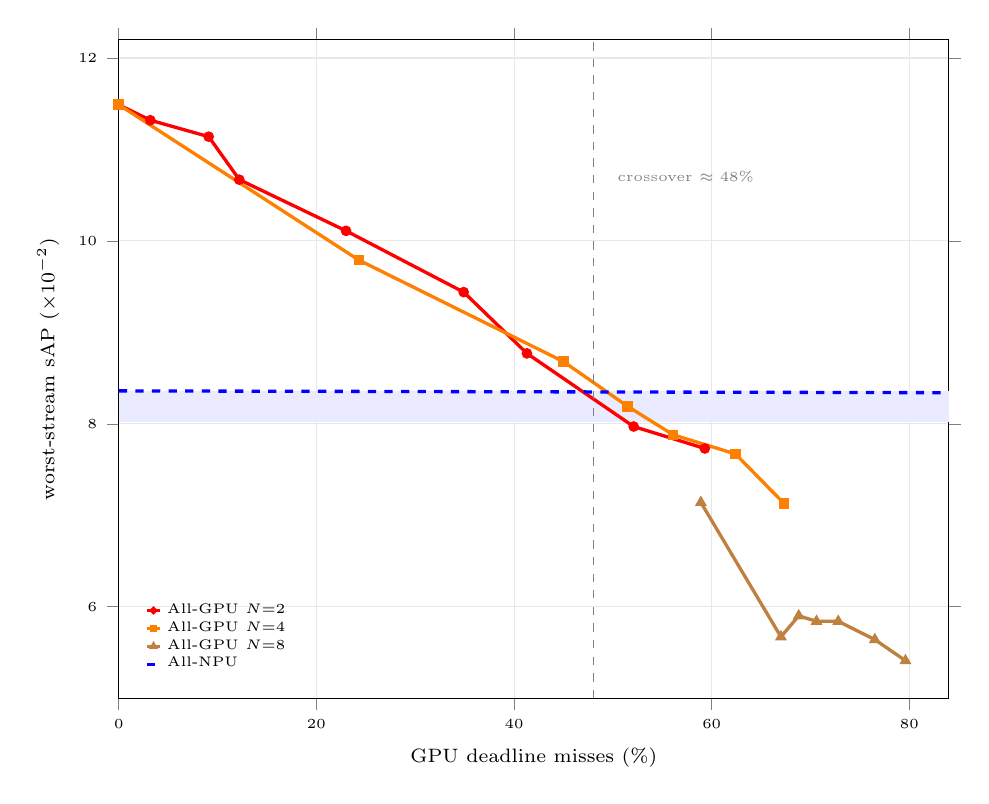
\begin{tikzpicture}
\begin{axis}[
  width=\linewidth, height=0.82\linewidth,
  xlabel={GPU deadline misses (\%)}, ylabel={worst-stream sAP ($\times10^{-2}$)},
  xmin=0, xmax=84, ymin=0.05, ymax=0.122,
  xtick={0,20,40,60,80}, ytick={0.06,0.08,0.10,0.12}, yticklabels={6,8,10,12},
  legend pos=south west, legend cell align=left, legend columns=1,
  legend style={font=\fontsize{1.3}{1.7}\selectfont, draw=none, line width=0.25pt,
    inner sep=0.5pt, row sep=-2.5pt,  fill=none},
  legend image post style={scale=0.55},
  legend image code/.code={\draw[#1,mark repeat=2,mark phase=2] plot coordinates {(0mm,0mm)(1.5mm,0mm)(3mm,0mm)};},
  grid=both, major grid style={gray!18}, tick align=outside,
  label style={font=\scriptsize}, tick label style={font=\tiny},
  every axis plot/.append style={very thick, mark size=1.3pt},
]
\fill[blue!8] (axis cs:0,0.0802) rectangle (axis cs:84,0.0836);
\addplot[red,    mark=*]         coordinates {(0.0,0.1149)(3.2,0.1132)(9.1,0.1114)(12.2,0.1067)(23.0,0.1011)(34.9,0.0944)(41.3,0.0877)(52.1,0.0797)(59.3,0.0773)};
\addlegendentry{All-GPU $N{=}2$}
\addplot[orange, mark=square*]   coordinates {(0.0,0.1149)(24.3,0.0979)(45.0,0.0868)(51.5,0.0819)(56.1,0.0788)(62.4,0.0767)(67.3,0.0713)};
\addlegendentry{All-GPU $N{=}4$}
\addplot[brown,  mark=triangle*] coordinates {(58.9,0.0714)(67.0,0.0567)(68.8,0.0590)(70.6,0.0584)(72.8,0.0584)(76.5,0.0564)(79.6,0.0541)};
\addlegendentry{All-GPU $N{=}8$}
\addplot[blue, dashed, mark=none] coordinates {(0,0.0836)(84,0.0834)};
\addlegendentry{All-NPU}
\draw[dashed,gray] (axis cs:48,0.05) -- (axis cs:48,0.122);
\node[anchor=west,gray,font=\tiny] at (axis cs:49.5,0.107) {crossover $\approx48\%$};
\end{axis}
\end{tikzpicture}
\caption{Homogeneous policies for $N{=}2,4,8$. The dashed All-NPU line is for $N{=}4$; the shaded band spans the All-NPU values across $N{=}2,4,8$.}
\label{fig:sweep}
\end{subfigure}
\hfill
\begin{subfigure}[t]{0.49\textwidth}
\centering
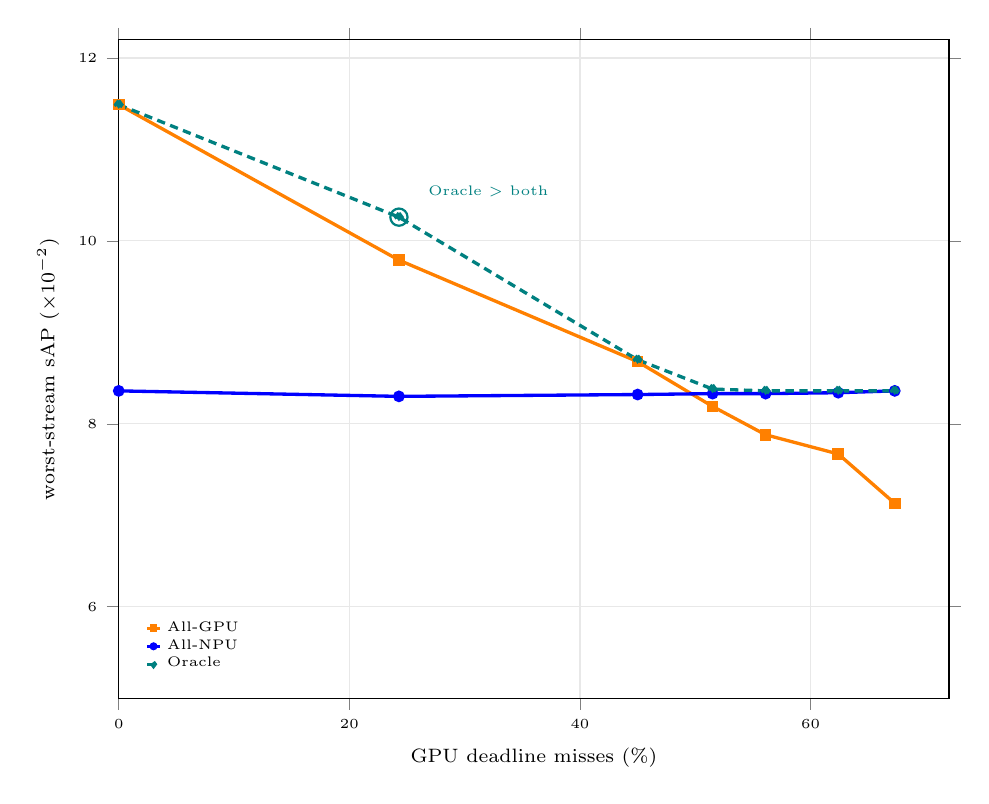
\begin{tikzpicture}
\begin{axis}[
  width=\linewidth, height=0.82\linewidth,
  xlabel={GPU deadline misses (\%)}, ylabel={worst-stream sAP ($\times10^{-2}$)},
  xmin=0, xmax=72, ymin=0.05, ymax=0.122,
  xtick={0,20,40,60}, ytick={0.06,0.08,0.10,0.12}, yticklabels={6,8,10,12},
  legend pos=south west, legend cell align=left,
  legend style={font=\fontsize{1.3}{1.7}\selectfont, draw=none, line width=0.25pt, inner sep=0.5pt, row sep=-2.5pt,  fill=none},
  legend image post style={scale=0.55},
  legend image code/.code={\draw[#1,mark repeat=2,mark phase=2] plot coordinates {(0mm,0mm)(1.5mm,0mm)(3mm,0mm)};},
  grid=both, major grid style={gray!18}, tick align=outside,
  label style={font=\scriptsize}, tick label style={font=\tiny},
  every axis plot/.append style={very thick, mark size=1.5pt},
]
\addplot[orange, mark=square*] coordinates {(0.0,0.1149)(24.3,0.0979)(45.0,0.0868)(51.5,0.0819)(56.1,0.0788)(62.4,0.0767)(67.3,0.0713)};
\addlegendentry{All-GPU}
\addplot[blue, mark=*] coordinates {(0.0,0.0836)(24.3,0.0830)(45.0,0.0832)(51.5,0.0833)(56.1,0.0833)(62.4,0.0834)(67.3,0.0836)};
\addlegendentry{All-NPU}
\addplot[teal, mark=diamond*, densely dashed] coordinates {(0.0,0.1149)(24.3,0.1026)(45.0,0.0870)(51.5,0.0838)(56.1,0.0836)(62.4,0.0836)(67.3,0.0836)};
\addlegendentry{Oracle}
\node[circle,draw=teal,thick,inner sep=2.2pt] at (axis cs:24.3,0.1026){};
\node[anchor=south west,teal,font=\tiny] at (axis cs:26,0.1038){Oracle $>$ both};
\end{axis}
\end{tikzpicture}
\caption{All-GPU, All-NPU, and diagnostic Oracle under mixed placements, $N{=}4$.}
\label{fig:split}
\end{subfigure}
\caption{Worst-stream sAP versus GPU deadline misses under GPU-localized contention (ResNet50 co-tenant). All-GPU degrades with increasing GPU staleness, while All-NPU remains stable. The homogeneous-placement crossover occurs before full GPU saturation for $N{=}4$ and is consistent with the $N{=}2,8$ trends. The GPU-saturating VLM co-tenant, where All-GPU collapses further, is reported in Table~\ref{tab:main}.}
\label{fig:sweeps}
\end{figure}


\subsection{Placement Reversal Under Deployment-Time Contention}
\label{sec:results:reversal}

\paragraph{\textbf{The ranking observed in isolation can reverse under contention.}}
Table~\ref{tab:main} compares worst-stream sAP across deployment configurations.
Although isolated profiling favors GPU execution because the NPU incurs an INT8 quantization penalty, the deployment-time ranking changes when contention affects the GPU path.
In that setting, GPU-induced staleness can exceed the NPU's quantization loss, making All-NPU preferable despite its lower isolated accuracy.

The clearest reversal occurs at the \Lvlm{} endpoint in Table~\ref{tab:main}.
All-GPU falls to a worst-stream sAP of $0.016$, while All-NPU maintains $0.083$, giving a $5.2\times$ gap.
The Oracle matches All-NPU at this endpoint, indicating that no mixed placement in the restricted Oracle family improves the worst-stream score.
This reversed ranking remains stable across repeated high-contention runs.
Figure~\ref{fig:sweeps} shows that this reversal appears before the GPU-saturating \Lvlm{} endpoint.
As GPU deadline misses increase in the ResNet50 co-tenant sweep, All-GPU steadily degrades, while All-NPU remains nearly constant.
The resulting crossover shows that complete GPU saturation is not required for the isolated ranking to reverse.

\paragraph{\textbf{The reversal depends on which resource is saturated.}}
The reversal is not caused by contention alone. Table~\ref{tab:main} shows that the outcome depends on which path is bottlenecked. Under the light CNN co-tenant, GPU placements remain competitive and no clear reversal is observed. Under the \Llm{} co-tenant, both paths are stressed: GPU deadline misses reach $83\%$ and NPU deadline misses reach $76\%$, so All-GPU still wins in worst-stream sAP despite substantial GPU contention. In contrast, under the \Lvlm{} co-tenant, GPU deadline misses reach $100\%$ while NPU deadline misses remain $1\%$, and the ranking reverses in favor of All-NPU. In our measurements, host CPU utilization rises from $17\%$ to $93\%$ under the \Llm{} co-tenant, stalling NPU host-side post-processing.
%
This is consistent with our earlier finding that NPU single-stream latency is dominated by host-side post-processing rather than on-chip inference, so CPU contention (not GPU contention) stalls the NPU path.


\begin{table}
\centering
\caption{Worst-stream and mean sAP at $N{=}4$ under GPU co-tenancy. The DM column reports All-GPU GPU deadline misses and All-NPU NPU deadline misses (\%).}
\label{tab:main}
\setlength{\tabcolsep}{5pt}
\begin{tabular}{lcc|cc|cc|c}
\toprule
 & \multicolumn{2}{c|}{All-GPU} & \multicolumn{2}{c|}{All-NPU} & \multicolumn{2}{c|}{Oracle} & GPU/NPU \\
co-tenant & worst & mean & worst & mean & worst & mean & DM (\%) \\
\midrule
\Lcnn{} (ResNet)   & $0.098$ & $0.137$ & $0.083$ & $0.126$ & $0.103$ & $0.137$ & $24 / 1$ \\
\Llm{} ($+$LLM)   & $0.062$ & $0.100$ & $0.042$ & $0.088$ & $0.063$ & $0.099$ & $83 / 76$ \\
\Lvlm{} ($+$VLM)  & $0.016$ & $0.047$ & $0.083$ & $0.126$ & $0.083$ & $0.120$ & $100 / 1$ \\
\bottomrule
\end{tabular}
\end{table}




% \begin{figure} [tb]
% \centering
% \begin{subfigure}[t]{0.49\textwidth}
% \centering
% \begin{tikzpicture}
% \begin{axis}[
%   width=\linewidth, height=0.82\linewidth,
%   xlabel={GPU deadline misses (\%)}, ylabel={worst-stream sAP ($\times10^{-2}$)},
%   xmin=0, xmax=103, ymin=0.01, ymax=0.122,
%   xtick={0,20,40,60,80,100}, ytick={0.02,0.04,0.06,0.08,0.10,0.12}, yticklabels={2,4,6,8,10,12},
%   legend pos=south west, legend cell align=left, legend columns=1,
%   legend style={font=\fontsize{1.3}{1.7}\selectfont, draw=none, line width=0.25pt,
%     inner sep=0.5pt, row sep=-2.5pt,  fill=none},
%   legend image post style={scale=0.55},
%   legend image code/.code={\draw[#1,mark repeat=2,mark phase=2] plot coordinates {(0mm,0mm)(1.5mm,0mm)(3mm,0mm)};},
%   grid=both, major grid style={gray!18}, tick align=outside,
%   label style={font=\scriptsize}, tick label style={font=\tiny},
%   every axis plot/.append style={very thick, mark size=1.3pt},
% ]
% \fill[blue!8] (axis cs:0,0.0802) rectangle (axis cs:100,0.0836);
% \addplot[red,    mark=*]         coordinates {(0.0,0.1149)(3.2,0.1132)(9.1,0.1114)(12.2,0.1067)(23.0,0.1011)(34.9,0.0944)(41.3,0.0877)(52.1,0.0797)(59.3,0.0773)};
% \addlegendentry{All-GPU $N{=}2$}
% \addplot[orange, mark=square*]   coordinates {(0.0,0.1149)(24.3,0.0979)(45.0,0.0868)(51.5,0.0819)(56.1,0.0788)(62.4,0.0767)(67.3,0.0713)};
% \addlegendentry{All-GPU $N{=}4$}
% \addplot[brown,  mark=triangle*] coordinates {(58.9,0.0714)(67.0,0.0567)(68.8,0.0590)(70.6,0.0584)(72.8,0.0584)(76.5,0.0564)(79.6,0.0541)};
% \addlegendentry{All-GPU $N{=}8$}
% \addplot[blue, dashed, mark=none] coordinates {(0,0.0836)(100,0.0833)};
% \addlegendentry{All-NPU}
% % --- VLM-saturated All-GPU endpoints (100% GPU skip; co-tenant = VLM, not ResNet); stars color-matched to N, no connectors ---
% \addplot[red,    only marks, mark=star, mark size=2.2pt, forget plot] coordinates {(100,0.0181)};
% \addplot[orange, only marks, mark=star, mark size=2.2pt, forget plot] coordinates {(100,0.0159)};
% \addplot[brown,  only marks, mark=star, mark size=2.2pt, forget plot] coordinates {(98.9,0.0136)};
% \addlegendimage{black, only marks, mark=star, mark size=4pt, mark options={line width=0.4pt}}
% \addlegendentry{All-GPU VLM sat.\ (100\%)}
% \draw[dashed,gray] (axis cs:48,0.01) -- (axis cs:48,0.122);
% \node[anchor=west,gray,font=\tiny] at (axis cs:49.5,0.107) {crossover $\approx48\%$};
% \end{axis}
% \end{tikzpicture}
% \caption{Homogeneous policies for $N{=}2,4,8$. The dashed All-NPU line is for $N{=}4$; the shaded band shows the All-NPU range over $N{=}2,4,8$.}
% \label{fig:sweep}
% \end{subfigure}
% \hfill
% \begin{subfigure}[t]{0.49\textwidth}
% \centering
% \begin{tikzpicture}
% \begin{axis}[
%   width=\linewidth, height=0.82\linewidth,
%   xlabel={GPU deadline misses (\%, All-GPU)}, ylabel={worst-stream sAP ($\times10^{-2}$)},
%   xmin=0, xmax=103, ymin=0.01, ymax=0.122,
%   xtick={0,20,40,60,80,100}, ytick={0.02,0.04,0.06,0.08,0.10,0.12}, yticklabels={2,4,6,8,10,12},
%   legend pos=south west, legend cell align=left,
%   legend style={font=\fontsize{1.3}{1.7}\selectfont, draw=none, line width=0.25pt, inner sep=0.5pt, row sep=-2.5pt,  fill=none},
%   legend image post style={scale=0.55},
%   legend image code/.code={\draw[#1,mark repeat=2,mark phase=2] plot coordinates {(0mm,0mm)(1.5mm,0mm)(3mm,0mm)};},
%   grid=both, major grid style={gray!18}, tick align=outside,
%   label style={font=\scriptsize}, tick label style={font=\tiny},
%   every axis plot/.append style={very thick, mark size=1.5pt},
% ]
% \addplot[orange, mark=square*] coordinates {(0.0,0.1149)(24.3,0.0979)(45.0,0.0868)(51.5,0.0819)(56.1,0.0788)(62.4,0.0767)(67.3,0.0713)};
% \addlegendentry{All-GPU}
% \addplot[blue, mark=*] coordinates {(0.0,0.0836)(24.3,0.0830)(45.0,0.0832)(51.5,0.0833)(56.1,0.0833)(62.4,0.0834)(67.3,0.0836)};
% \addlegendentry{All-NPU}
% \addplot[teal, mark=diamond*, densely dashed] coordinates {(0.0,0.1149)(24.3,0.1026)(45.0,0.0870)(51.5,0.0838)(56.1,0.0836)(62.4,0.0836)(67.3,0.0836)};
% \addlegendentry{Oracle}
% % --- VLM-saturated endpoint (100% GPU skip; co-tenant = VLM, not ResNet); only All-GPU starred, no connector ---
% \addplot[orange, only marks, mark=star, mark size=2.2pt, forget plot] coordinates {(100,0.0159)};
% \addlegendimage{orange, only marks, mark=star, mark size=4pt, mark options={line width=0.4pt}}
% \addlegendentry{All-GPU VLM sat.\ (100\%)}
% \node[circle,draw=teal,thick,inner sep=2.2pt] at (axis cs:24.3,0.1026){};
% \node[anchor=south west,teal,font=\tiny] at (axis cs:26,0.1038){Oracle $>$ both};
% \end{axis}
% \end{tikzpicture}
% \caption{All-GPU, All-NPU, and diagnostic Oracle under mixed placements, $N{=}4$.}
% \label{fig:split}
% \end{subfigure}
% \caption{Worst-stream sAP versus GPU deadline misses under GPU-localized contention. All-GPU degrades with increasing GPU staleness, while All-NPU remains stable. The homogeneous-placement crossover occurs before full GPU saturation for $N{=}4$ and is consistent with the $N{=}2,8$ trends. Stars mark VLM-saturated All-GPU endpoints; all other points use the ResNet50 co-tenant.}
% \label{fig:sweeps}
% \end{figure}



\paragraph{\textbf{GPU-localized contention reveals a crossover and a useful split placement.}}

Figure~\ref{fig:sweeps} examines the complementary case where GPU-bound ResNet50 co-tenants localize contention to the GPU path. The NPU path remains largely unaffected, with NPU deadline-miss rate never exceeding $4.0\%$. As contention increases, All-GPU worst-stream sAP decreases monotonically, while All-NPU stays nearly constant. For the $N{=}4$ All-GPU curve, the All-GPU and All-NPU worst-stream curves cross at about $48\%$ GPU deadline-miss rate. This reversal pattern is not specific to $N{=}4$. In Fig.~\ref{fig:sweeps}a, the All-GPU curve crosses the All-NPU level at about $47$--$48\%$ GPU deadline-miss rate for $N{=}2$ and $N{=}4$, while for $N{=}8$ the All-GPU curve is already below the All-NPU level at the lowest measured ResNet50 contention point. Across $N{=}2,4,8$, All-NPU remains confined to a narrow band around $0.083$, indicating that the reversal is driven primarily by GPU-localized staleness rather than by a changing NPU baseline.

The same sweep also explains why we use deadline misses, rather than aggregate GPU utilization, as the contention coordinate. After a ResNet50 co-tenant is introduced, average GPU utilization remains nearly flat at about $68\%$, while the foreground GPU deadline-miss rate rises from $24.3\%$ to $67.3\%$. The placement reversal therefore follows missed real-time deadlines rather than aggregate GPU utilization.

Figure~\ref{fig:sweeps}b shows that neither homogeneous policy is optimal across the full GPU-localized contention sweep. All-GPU is best at low contention because the NPU's quantization loss dominates. All-NPU is best at high contention because GPU-resident streams suffer severe staleness. At low-to-moderate contention (about $24\%$ GPU deadline-miss rate), the Oracle-selected placement is the large-object-aware one-stream split, with a worst-stream sAP of $0.103$. This slightly exceeds All-GPU at $0.098$ and All-NPU at $0.083$. The split helps because moving the most affected large-object stream to the NPU removes it from GPU-induced staleness and reduces contention on the remaining GPU streams.

Overall, the preferred placement changes with the contention level, and the crossover occurs before complete GPU saturation.



\paragraph{\textbf{QoS mitigates contention but does not remove the reversal.}}
\label{sec:results:qos}

A natural objection is that the reversal merely reflects unmanaged scheduling, and that prioritizing foreground GPU inference would remove it. We therefore test whether CUDA stream priority eliminates the reversal by assigning all foreground inference to a maximum-priority CUDA stream and repeating the $N{=}4$ contention sweep. QoS improves foreground latency and worst-stream sAP, but it does not restore uncontended behavior. Under the GPU-saturating VLM co-tenant, All-NPU (worst-stream sAP $0.083$) still outperforms protected All-GPU ($0.033$) by $2.5\times$. QoS therefore shifts the crossover to heavier contention but does not eliminate placement reversal.


\begin{table}%[tb]
\centering
\caption{Metric sensitivity at a high-contention ResNet50 sweep point. Mean and median mask the degraded camera, whereas worst-stream and lower-tail statistics expose it. Percentiles use linear interpolation, so at $N{=}4$ the $10$th percentile lies just above the worst stream.}
\label{tab:metric-sensitivity}
\setlength{\tabcolsep}{8pt}
\begin{tabular}{lccc}
\toprule
statistic & All-GPU & All-NPU & exposes degraded camera? \\
\midrule
mean      & $0.107$ & $0.126$ & hides \\
median    & $0.087$ & $0.115$ & partial \\
$p_{10}$  & $0.072$ & $0.091$ & exposes \\
worst     & $0.066$ & $0.084$ & exposes \\
\bottomrule
\end{tabular}
\end{table}

\subsection{Mean sAP Understates the Worst Camera}
\label{sec:results:worst}

Table~\ref{tab:main} shows a substantial gap between mean and worst-stream sAP under contention. Under the VLM co-tenant, All-GPU achieves a mean sAP of $0.047$. Its worst-stream sAP is only $0.016$, so the mean is $2.9\times$ the worst-stream score. In contrast, All-NPU exhibits a much smaller gap. It achieves $0.126$ mean sAP and $0.083$ worst-stream sAP. The gap therefore reflects how unevenly contention is distributed across cameras.

The effect can also appear in non-oracle mixed placements that leave some cameras on the saturated GPU. In such cases, the cameras remaining on the GPU can dominate the worst-case behavior even when the mean improves. The mean therefore substantially understates the worst affected camera.

This masking also appears at a high-contention ResNet50 sweep point, distinct from the VLM endpoint, as summarized in Table~\ref{tab:metric-sensitivity}. Both the mean and median remain substantially above the worst-stream score. Only lower-tail metrics track the degraded camera. At $N{=}4$, $p_{10}$ nearly coincides with the worst stream and reaches the same conclusion. The mean is $1.6\times$ the worst-stream score. Removing the worst camera raises the system mean from $0.107$ to $0.121$ at $N{=}4$.
Central-tendency metrics therefore understate failures concentrated in a single stream. This matters because a single severely degraded camera can compromise the multi-camera perception system.


Finally, the worst-stream score is not determined only by stream content. In our runs, the same stream is usually the worst across the compared placements, but its degradation becomes much larger when it runs on the contended GPU. Under All-NPU, its score stays nearly unchanged. Worst-stream sAP therefore captures contention-induced degradation, not just differences among streams.

% ===============================================================
\section{Discussion}
\label{sec:discussion}

\subsection{Implications for Streaming-Perception Evaluation}
\label{sec:discussion:evaluation}

Our results concern how streaming perception is evaluated. The field commonly reports a single aggregate sAP measured on one camera in isolation. We show that this signal can recommend a placement that becomes suboptimal under deployment-relevant co-tenancy. Averaging across cameras can also conceal a severely degraded stream.

\paragraph{\textbf{A deployment-faithful reporting protocol.}}

We do not propose a general robustness framework. Instead, we distill our findings into three reporting recommendations for shared platforms. First, report sAP under co-tenancy localized to the shared accelerator, not only in isolation. Second, report worst-stream sAP alongside mean sAP. Third, report the contention sweep and crossover point. These measurements expose the reversal and its severity. The standard isolated single-stream evaluation protocol hides both. Table~\ref{tab:reporting} summarizes the contrast.



\begin{table}[tb]
\centering
\caption{Conventional versus deployment-faithful streaming-perception reporting.}
\label{tab:reporting}
\setlength{\tabcolsep}{8pt}
\begin{tabular}{ll}
\toprule
Conventional reporting & Deployment-faithful reporting \\
\midrule
isolated single-stream sAP   & co-tenancy-aware multi-stream sAP \\
mean sAP only                & mean $+$ worst-stream sAP \\
aggregate GPU utilization    & foreground deadline-miss rate \\
single operating point       & contention sweep $+$ crossover point \\
\bottomrule
\end{tabular}
\end{table}

\paragraph{\textbf{Why worst-stream rather than another tail metric?}}

Worst-stream is not the only valid lower-tail statistic. Percentile, CVaR, and min-$k$ metrics would reveal the same degraded camera. We use worst-stream because it matches the semantics of a multi-camera perception loop. In such a loop, one severely degraded stream can compromise the system. Worst-stream is also well suited to small-$N$ deployments. Percentile and CVaR estimates become coarse in this setting. In our $N{=}4$ setting, the $10$th percentile nearly coincides with the minimum. Worst-stream therefore provides a simple and stable lower-tail summary.

\subsection{Limitations}
\label{sec:discussion:limitations}

\noindent\textbf{Detector and toolchain coverage.}
Our main results use YOLOv11s, and the same reversal appears on YOLOv8n, YOLOv8s, YOLOv10s, and YOLO12s, with detector-dependent crossover points in Table~\ref{tab:detector-generality}. Coverage nevertheless remains limited to the YOLO family, and validation on larger and non-YOLO architectures remains future work.

The reversal is conditional on size-dependent quantization loss. In our experiments, INT8 loss is concentrated on small objects, while large objects are mainly limited by GPU staleness. This qualitative pattern is broadly consistent across the YOLO-family detectors we evaluated, although the magnitude of the large-object INT8 loss and the crossover point are detector-dependent.

A fine-tuned YOLOv11s model shows the same trend across the tested export settings. Small-object loss remains significant, ranging from $-43\%$ to $-35\%$ ($p<0.001$), whereas the large-object change remains statistically insignificant. The absolute loss values from this probe are not directly comparable to Table~\ref{tab:single-stream} because they use different export configurations.

\begin{table}
\centering
\caption{Cross-detector reproduction of the placement reversal. The table summarizes isolated size-bin preference, VLM worst-stream sAP, and the contention-sweep crossover point.}
\label{tab:detector-generality}
\setlength{\tabcolsep}{4pt}
\begin{tabular}{lccccc}
\toprule
Detector & isolated small & isolated large & VLM cont. & worst NPU/GPU & cross. \\
\midrule
YOLO12s  & GPU ($-36\%$) & tie ($-1.2\%$) & NPU & $0.080/0.011$ & $\approx45\%$ \\
YOLOv11s & GPU ($-48\%$) & tie ($+0.1\%$) & NPU & $0.083/0.016$ & $\approx48\%$ \\
YOLOv10s & GPU ($-45\%$) & GPU ($-4.6\%$) & NPU & $0.082/0.016$ & $\approx30\%$ \\
YOLOv8s  & GPU ($-44\%$) & tie ($-0.3\%$) & NPU & $0.080/0.015$ & $\approx31\%$ \\
YOLOv8n  & GPU ($-36\%$) & GPU ($-8.1\%$) & NPU & $0.060/0.009$ & $\approx36\%$ \\
\bottomrule
\end{tabular}
\end{table}

\noindent\textbf{Measurement stability.}
Each reported value is averaged over at least three repeats. The single-stream size gaps and the VLM reversal remained stable across runs, with the VLM reversal showing a standard deviation below $0.001$. The light \Lcnn{} co-tenant at $N{=}4$ operates near the $33.3$~ms frame deadline, with a mean deadline margin of $-5.7$~ms. Its realized deadline-miss rate therefore varies across runs. To check this boundary case, we repeated it ten times. The GPU deadline-miss rate was $24.3 \pm 2.2\%$, All-GPU worst-stream sAP was $0.098 \pm 0.004$, and the large-object-aware one-stream split reached $0.103 \pm 0.003$. This split was selected in nine of ten runs. The light co-tenant therefore does not produce a homogeneous reversal, and this boundary variability does not alter the overall pattern.

\noindent\textbf{The NPU accuracy ceiling.}
Even under the best placement, performance remains bounded by the NPU's INT8 accuracy loss. Moving cameras to the NPU avoids GPU contention but does not recover quantization loss. Improving this bound requires techniques such as quantization-aware training or mixed-precision inference.

\noindent\textbf{Platform and workload scope.}
We evaluate a single NPU vendor and card, and emulate multi-camera workloads by replaying distinct single-camera Argoverse-HD logs. The degree of NPU isolation from GPU contention is platform-dependent. Discrete accelerators may be more isolated, whereas SoC-integrated NPUs may share memory bandwidth with the GPU. Thus, the placement-reversal mechanism may extend to other platforms, but crossover points and placement decisions remain hardware-dependent. Validation on synchronized multi-camera benchmarks with streaming labels remains future work.
% ===============================================================


\section{Conclusion}
\label{sec:conclusion}

We showed that isolated streaming-perception evaluation can mis-rank accelerator placement on a heterogeneous GPU--NPU platform. In isolation, the FP32 GPU is preferred because the INT8 NPU loses accuracy mainly on small objects. Under deployment-time contention, however, GPU deadline misses introduce staleness that mainly hurts medium and large objects. This shift in the dominant loss mechanism can reverse the placement ranking before complete GPU saturation. The reversal also depends on whether the bottleneck affects GPU execution or host-side CPU post-processing, so placement cannot be inferred from isolated accuracy or aggregate GPU utilization alone.

In the ResNet50 sweep, foreground deadline misses track the reversal more directly than aggregate GPU utilization, and a simple split placement helps at low-to-moderate contention. Under the GPU-saturating \Lvlm{} co-tenant, All-NPU improves worst-stream sAP over All-GPU by $5.2\times$. We also showed that mean sAP can hide severe degradation in one stream, while worst-stream sAP exposes this failure directly. Deployment-faithful streaming-perception evaluation should therefore report co-tenancy-aware contention sweeps, foreground deadline-miss rates, crossover points, and worst-stream sAP alongside mean sAP.





% ===============================================================
% =============== APPENDIX (commented out) ======================
% Uncomment the block below to include the appendix in the build.
% Contains the full per-size All-GPU contention table relocated from
% Sec.~\ref{sec:results:decomp} to save space in the main text.
%
% \appendix
% \section{Per-size contention loss}
% \label{app:persize}
%
% \begin{table}[tb]
% \centering
% \caption{Per-size All-GPU sAP loss under ResNet50 contention ($N{=}4$, YOLOv11s). Losses are relative to the no-contention All-GPU baseline. This is the tabular form of the size-dependent pattern plotted in Fig.~\ref{fig:persize-sweep}.}
% \label{tab:persize-contention}
% \setlength{\tabcolsep}{7pt}
% \begin{tabular}{lccc}
% \toprule
% \multirow{2}{*}{GPU deadline-miss rate} & \multicolumn{3}{c}{sAP loss} \\
% \cmidrule(lr){2-4}
%  & Small & Medium & Large \\
% \midrule
% $\approx24\%$ & $0.000$ & $0.017$ & $0.042$ \\
% $\approx45\%$ & $0.001$ & $0.032$ & $0.078$ \\
% $\approx56\%$ & $0.002$ & $0.040$ & $0.096$ \\
% $\approx67\%$ & $0.002$ & $0.046$ & $0.120$ \\
% \bottomrule
% \end{tabular}
% \end{table}
%
% \begin{table}[tb]
% \centering
% \caption{Per-size All-NPU sAP across the ResNet50 $k$-sweep ($N{=}4$, YOLOv11s), where $k$ is the number of GPU-pinned ResNet50 co-tenants. Because the NPU uses a separate compute path, its realized deadline-miss rate stays below $1.4\%$ and per-size sAP is essentially flat. The maximum change across the sweep is $0.0001$ (small), $0.0007$ (medium), and $0.0021$ (large), confirming that the GPU-localized contention sweep does not perturb the NPU path. This is the All-NPU counterpart to Table~\ref{tab:persize-contention}.}
% \label{tab:persize-npu}
% \setlength{\tabcolsep}{7pt}
% \begin{tabular}{lccc}
% \toprule
% $k$ & Small & Medium & Large \\
% \midrule
% $0$ & $0.0035$ & $0.1305$ & $0.4327$ \\
% $1$ & $0.0035$ & $0.1297$ & $0.4307$ \\
% $2$ & $0.0035$ & $0.1302$ & $0.4322$ \\
% $3$ & $0.0036$ & $0.1303$ & $0.4321$ \\
% $4$ & $0.0036$ & $0.1303$ & $0.4326$ \\
% $6$ & $0.0036$ & $0.1300$ & $0.4328$ \\
% $8$ & $0.0036$ & $0.1304$ & $0.4320$ \\
% \bottomrule
% \end{tabular}
% \end{table}
%
% \begin{table}[tb]
% \centering
% \caption{Diagnostic system counters for the ResNet50 contention sweep ($N{=}4$, All-GPU, mean over repeated runs). Here $k$ denotes the number of GPU-pinned ResNet50 co-tenants. GPU utilization stays near $68\%$ once co-tenants are present, whereas foreground deadline-miss rate continues to increase.}
% \label{tab:gpu-util}
% \setlength{\tabcolsep}{6pt}
% \begin{tabular}{lccccc}
% \toprule
% $k$ & GPU DM & util mean & util p95 & mem (MiB) & power (W) \\
% \midrule
% 0 & $0.0\%$  & $52\%$ & $71\%$ & $3012$ & $178$ \\
% 1 & $24.3\%$ & $70\%$ & $86\%$ & $3155$ & $238$ \\
% 2 & $45.0\%$ & $66\%$ & $79\%$ & $3698$ & $247$ \\
% 3 & $51.5\%$ & $68\%$ & $79\%$ & $4233$ & $259$ \\
% 4 & $56.1\%$ & $68\%$ & $80\%$ & $5028$ & $267$ \\
% 6 & $62.4\%$ & $68\%$ & $80\%$ & $6088$ & $285$ \\
% 8 & $67.3\%$ & $69\%$ & $80\%$ & $7606$ & $300$ \\
% \bottomrule
% \end{tabular}
% \end{table}
% ===============================================================

% ===============================================================
\bibliographystyle{splncs04}
\bibliography{main}

\end{document}